\section{Cross Validation} 

  We have understood the theoretical foundations of overfitting and underfitting with the bias variance decomposition. But in practice, we don't have an ensemble of datasets; we just have one. Therefore, we don't actually know what the bias, the variance, or the noise is at all. Therefore, how do we actually \textit{know} in practice when we are underfitting or overfitting? Easy. We just split our dataset into 2 different parts: the training set and testing sets. 
  \begin{equation}
    \mathcal{D} = \mathcal{D}_{train} \sqcup \mathcal{D}_{test}
  \end{equation}
  What we usually have is a \textbf{training set} that allows us to train the model, and then to check its performance we have a \textbf{test set}. We would train the model on the training set, where we will always minimize the loss, and then we would look at the loss on the test set. Though we haven't made a testing set, since we know the true model let us just generate more data and use that as our testing set. For each model, we can calculate the optimal $\boldsymbol{\theta}$, which we will denote $\boldsymbol{\theta}^\ast$, according to the \textbf{root mean squared loss}
  \begin{equation}
    h_{\boldsymbol{\theta}^\ast} = \argmin_{h_{\boldsymbol{\theta}}} \sqrt{ \frac{1}{N} \sum_{i=1}^N \big( y^{(i)} - h_{\boldsymbol{\theta}} (\mathbf{x}^{(i)}) \big)^2 }
  \end{equation}
  where division of $N$ allows us to compare different sizes of datasets on equal footing, and the square root ensures that this is scaled correctly. Let us see how well these different order models perform on a separate set of data generated by the same function with Gaussian noise. 

  \begin{figure}[H]
    \centering
    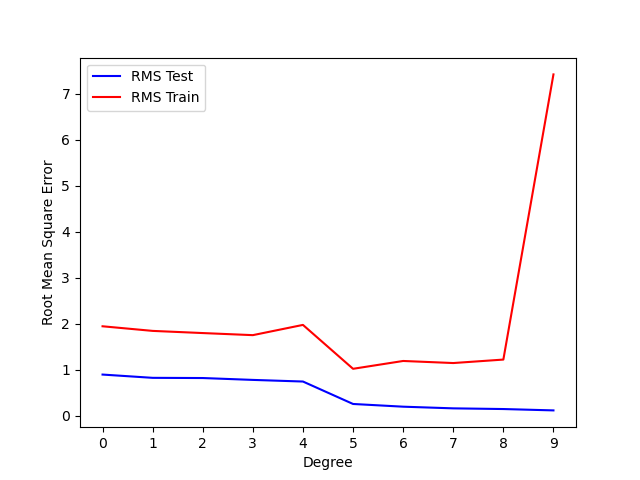
\includegraphics[scale=0.4]{img/Degree_vs_RMS.png}
    \caption{We can see that the RMS decreases monotonically on the training error as more complex functions become more fine-tuned to the data. However, when we have a $9$th degree polynomial the RMS for the testing set dramatically increases, meaning that this model does not predict the testing set well, and performance drops. }
    \label{fig:poly_deg_vs_rms}
  \end{figure}

  Now we know that a more complex model (i.e. that captures a greater set of functions) is not necessarily the best due to overfitting. Therefore, researchers perform \textbf{cross-validation} by taking the training set $(\mathcal{X}, \mathcal{Y})$. We divide it into $S$ equal pieces 
  \begin{equation}
    \bigcup_{s=1}^S D_s = (\mathcal{X}, \mathcal{Y})
  \end{equation}
  Then, we train the model $\mathcal{M}$ on $S-1$ pieces of the data and then test it across the final piece, and do this $S$ times for every test piece, averaging its perforance across all $S$ test runs. Therefore, for every model $\mathcal{M}_k$, we must train it $S$ times, for all $K$ models, requiring $KS$ training runs. If data is particularly scarce, we set $S = N$, called the \textbf{leave-one-out} technique. Then we just choose the model with the best average test performance. 

  \begin{code}[Minimal Example of Train Test Split in scikit-learn]
    To implement this in scikit-learn, we want to use the \texttt{train\_test\_split} class. We can also set a random state parameter to reproduce results. 
    \begin{lstlisting}
      from sklearn.model_selection import train_test_split 

      # Split into training (80\%) and test (20\%) data 
      X_train, X_test, Y_train, Y_test = train_test_split(X, Y, test_size=0.2, random_state=66)
    \end{lstlisting}
  \end{code}

\subsection{Concentration Bounds}

  The following result shows that cross-validation (data splitting) leads to an estimator with risk nearly as good as the best model in the class. 

  \begin{theorem}[Gyorfi, Kohler, Krzyak, Walk (2002)]
    Let $\mathcal{M} = \{m_h\}$ be a finite class of regression estimators indexed by a parameter $h$, with $m$ being the true risk minimizer, $m_{\hat{h}}$ being the empirical risk minimizer over the whole dataset $\mathcal{D}$, and $m_{H}$ being the empirical risk minimizer over the test set $\mathcal{D}_{\mathrm{test}}$ for ordinary least squares loss. 
    \begin{align}
      m_H & = \argmin_{m_h} \frac{1}{N} \sum_{i \in \mathcal{D}_{\mathrm{test}}} (y_i - m_h(x_i))^2 \\ 
      m_{\hat{h}} & = \argmin_{m_h} \frac{1}{N} \sum_{i \in \mathcal{D}} (y_i - m_h(x_i))^2 
    \end{align}
    If the data $Y_i$ and estimators are bounded by $L$, then for any $\delta > 0$, we have 
    \begin{equation}
      \mathbb{E} \int |m_H (x) - m(x)|^2 \,d\mathbb{P}(x) \leq (1 + \delta) \mathbb{E} \int |m_{\hat{h}} (x) - m(x) |^2 \,d \mathbb{P}(x) + \frac{C (1 + \log{|M|})}{n}
    \end{equation}
    where $c = L^2 (16/\delta + 35 + 19\delta)$. 
  \end{theorem}
  \begin{proof}
    Then
    \begin{align}
      \mathbb{E} \left( \int |m_H - m|^2 dP(x)|D \right) &= \mathbb{E} \left( \int |Y - m_H|^2 dP(x)|D \right) - \mathbb{E}|Y - m(X)|^2 \\
      &= T_1 + T_2
    \end{align}
    where
    \begin{equation}
      T_1 = \mathbb{E} \left( \int |Y - m_H|^2 dP(x)|D \right) - \mathbb{E}|Y - m(X)|^2 - T_2
    \end{equation}
    and
    \begin{align}
      T_2 &= (1+\delta) \frac{1}{n} \sum_{D'} (|Y_i - m_H(X_i)|^2 - |Y_i - m(X_i)|^2) \\
      &\leq (1+\delta) \frac{1}{n} \sum_{D'} (|Y_i - m_{\hat{h}}(X_i)|^2 - |Y_i - m(X_i)|^2)
    \end{align}
    and so
    \begin{align}
      \mathbb{E}[T_2|D] &\leq (1 + \delta) \left( \mathbb{E}(|Y - m_{\hat{h}}(X)|^2|D) - \mathbb{E}|Y - m(X)|^2 \right) \\
      &= (1 + \delta) \int |m_{\hat{h}}(x) - m(x)|^2 dP(x).
    \end{align}

    The second part of the proof involves some tedious calculations. We will bound $P(T_1 \geq s|D)$. The event $T_1 \geq s$ is the same as
    \begin{align}
      &(1 + \delta) \left( \mathbb{E}(|m_H(X) - Y|^2|D) - \mathbb{E}|m(X) - Y|^2 - \frac{1}{n} \sum_{D'} (|Y_i - m_H(X_i)|^2 - |Y_i - m(X_i)|^2) \right) \\
      &\geq s + \delta \left( \mathbb{E}|m_H(X) - Y|^2 - \mathbb{E}|m(X) - Y|^2 \right).
    \end{align}

    This has probability at most $|\mathcal{M}|$ times the probability that
    \begin{align}
      &(1 + \delta) \left( \mathbb{E}(|m_h(X) - Y|^2|D) - \mathbb{E}|m(X) - Y|^2 - \frac{1}{n} \sum_{D'} (|Y_i - m_H(X_i)|^2 - |Y_i - m(X_i)|^2) \right) \\
      &\geq s + \delta \left( \mathbb{E}|m_h(X) - Y|^2 - \mathbb{E}|m(X) - Y|^2 \right)
    \end{align}
    for some $h$, that is
    \begin{equation}
      \mathbb{E}[Z|D] - \frac{1}{n} \sum_i Z_i \geq \frac{s + \delta\mathbb{E}[Z|D]}{1 + \delta}
    \end{equation}
    for some $h$, where $Z = |m_h(X) - Y|^2 - |m(X) - Y|^2$. Now
    \begin{equation}
      \sigma^2 = \text{Var}(Z|D) \leq \mathbb{E}[Z^2|D] \leq 16L^2 \int |m_h(x) - m(x)|^2 dP(x) = 16L^2 \mathbb{E}[Z|D].
    \end{equation}

    Using this, and Bernstein's inequality,
    \begin{align}
      P \left( \mathbb{E}[Z|D] - \overline{Z} \geq \frac{s + \delta\mathbb{E}[Z|D]}{1 + \delta} |D \right) \\
      \leq P \left( \mathbb{E}[Z|D] - \overline{Z} \geq \frac{s + \delta\sigma^2/(16L^2)}{1 + \delta} |D \right) \\
      \leq e^{-nA/B}
    \end{align}
    where
    \begin{equation}
      A = \frac{1}{(1 + \delta)^2} \left( s + \frac{\delta\sigma^2}{16L^2} \right)
    \end{equation}
    and
    \begin{equation}
      B = 2\sigma^2 + \frac{2 \cdot 8L^2}{3(1 + \delta)} \left( s + \frac{\delta\sigma^2}{16L^2} \right).
    \end{equation}

    Now $A/B \geq s/c$ for $c = L^2(16/\delta + 35 + 196)$. So
    \begin{equation}
      P(T_1 \geq s|D) \leq |\mathcal{M}| e^{-ns/c}.
    \end{equation}

    Finally
    \begin{equation}
      \mathbb{E}[T_1|D] \leq u + \int_u^{\infty} P(T_1 > s|D) \leq u + \frac{c|\mathcal{M}|}{n} e^{-nu/c}.
    \end{equation}

    The result follows by setting $u = c \log |\mathcal{M}|/n$. $\square$
  \end{proof}

\subsection{Leave 1 Out Cross Validation} 

  \subsubsection{Generalized (Approximate) Cross Validation} 

  \subsubsection{Cp Statistic}

\subsection{K Fold Cross Validation}

